\chapter{Wavelets}
\label{waveletsH}
De Fouriertransformatie bestaat al honderden jaren en is een grote speler geworden in de \emph{signal processing}. 
Een groot nadeel van deze transformatie is dat zij slecht reageert op discontinue signalen 
door de globale dragers van de basisfuncties. 
Hierdoor worden alle Fourierco\"effici\"enten be\"invloed door een discontinu\"iteit.
In de laatste dertig jaar is daarom een nieuwe transformatie ontwikkeld die beter blijkt om te gaan
met discontinu\"iteiten. We hebben het hier over de \emph{Wavelettransformatie}.

\begin{definitie}
  Een wavelet is simpelweg een functie $\psi: \R \to \R$ die voldoet aan
  \[
  \int_{-\infty}^{\infty} \psi(t) dt = 0.
  \]
  Met deze functie $\psi$ kunnen we een familie functies $\psi_{u,s}$ bouwen door middel van schaling en translatie:
  \[
  \psi_{u,s}(t) := \sqrt{s} \psi\left(s\cdot t-u\right).
  \]
\end{definitie}

Deze familie geeft aanleiding tot een Wavelettransformatie $W_f$ van $f$ in $(u,s)$:
\[
W_f(u,s) = \int_{-\infty}^\infty f(t) \psi^*_{u,s}(t) dt.
\]

Het is verder mogelijk om wavelets te construeren die met deze schaling en translatie een basis voor de $L_2(\R)$ vormen. 
Over het algemeen kijken we dan naar
\[
\left\{ \psi_{j,n}(t) = \sqrt{2^j} \psi\left( 2^j t - n\right) : (j,n) \in \Z^2 \right\}.
\]
De kunst is nu om de basiselementen loodrecht op elkaar te laten staan, zodat er een orthogonale 
(en met de juiste factoren zelfs een orthonormale) basis gevormd wordt. 
Zie figuur~\ref{fig:wavelets} voor twee wavelets.

\begin{figure}[h]
  \centering
  \begin{subfigure}{0.48\linewidth}
    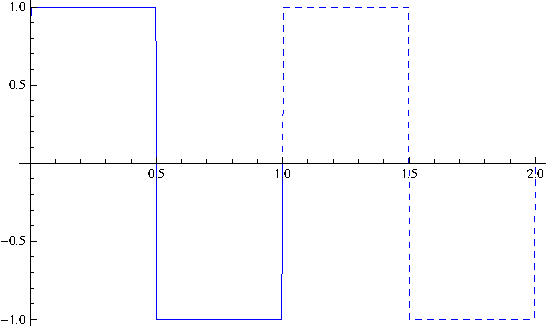
\includegraphics[width=\linewidth]{plaatjes/db1.pdf}
  \end{subfigure}
  \begin{subfigure}{0.48\linewidth}
    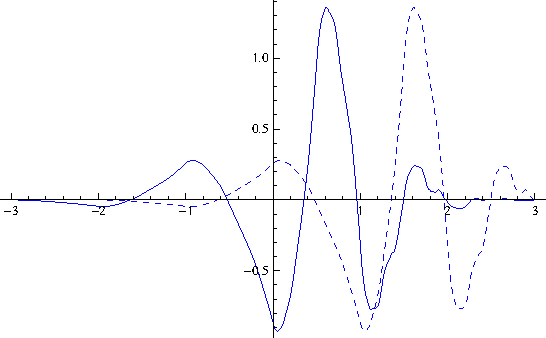
\includegraphics[width=\linewidth]{plaatjes/db4.pdf}
  \end{subfigure}
  \caption{Links: De Haarwavelet. Rechts: De Daubechies-2-wavelet. De gestippelde grafiek is een translatie naar rechts en staat in beide gevallen loodrecht op de continue lijn die de waveletfunctie voorstelt.}
\label{fig:wavelets}
\end{figure}

Het gedrag bij discontinuiteiten van de Fouriertransformatie maakt compressie van signalen met harde randen moeilijk. 
Veel wavelets worden daarom z\'o geconstrueerd dat dit probleem (deels) verholpen wordt. 
We zijn namelijk op zoek naar een wavelet die een eindige drager heeft. 
Het blijkt dat deze wavelets bestaan en dat er zelfs een hele grote verzameling van zulke wavelets is, 
elk met eigen gewilde eigenschappen.

Omdat wij naar de toepassing van wavelets binnen de beeldcompressie bekijken, 
zijn we natuurlijk vooral ge\"interesseerd in discrete toepassingen.
We kijken dus naar een benadering van een functie $f$. Hiervoor gebruiken we een rij geneste ruimtes die 
uiteindelijk naar de $L_2(\R)$ toe gaat:
\begin{equation}
  \label{multires}
  V_0 \subset V_1 \subset \ldots \subset L_2(\R).
\end{equation}
We noemen deze rij een multiresolutie.
\begin{definitie}
  Een rij geneste ruimtes $\{ V_j: j \in \N_0 \}$ zoals in~\eqref{multires} heet een multiresolutie wanneer voldaan wordt aan de volgende eigenschappen:
  \begin{eqnarray}
    \forall j, k: f(t) \in V_j \implies f(t - 2^j k) \in V_j, \\
    \forall j: V_{j-1} \subset V_j, \\
    \forall j: f(t) \in V_j \iff f(t/2) \in V_{j-1}, \\
    \bigcup_{j=0}^{\infty} V_j = \lim_{j\to\infty} V_j = L_2(\R), \\
    \text{ Er is $\phi: \R \to \R$ zo dat $\{ \phi(t-n): n \in \Z \}$ een orthonormale basis voor $V_0$ is.}
  \end{eqnarray}
\end{definitie}

\begin{voorbeeld} We bekijken een multiresolutie van ruimtes over stuksgewijs constante functies, 
  de ruimte $V_j$ die we hiervoor bekijken is:
  \[
  V_j = \left\{ g(t) \in L_2(\R) \largediv g(t)\text{ constant voor }t \in [n 2^{-j}, (n+1)2^{-j}) \right \}
    \text{ met } n \in \Z.
    \]
    De basisfunctie $\phi$ voor $V_0$ wordt in dit geval $\phi(t) = 1_{[0,1)}(t)$.
\end{voorbeeld}

\section{Schalingsfuncties}
Wanneer we nu een orthonormale basis hebben voor $V_0$, willen we graag een orthonormale basis voor $V_j$ construeren.
\begin{stelling}[{\cite[T7.1]{mallat}}]
  Laat $\{ V_j \}$ een multiresolutie en laat $\{\phi(t-n) \}$ de basis voor $V_0$. Laat verder
  \[
  \phi_{j,n}(t) := \sqrt{2^j} \phi\left( t2^j - n \right).
  \]
  Dan is $\{ \phi_{j,n}: n \in \Z \}$ een orthonormale basis voor $V_j$. 
\end{stelling}
De functie $\phi$ heet ook wel de \emph{schalingsfunctie}.
\subsection{Benadering} De orthogonale projectie van $f$ op $V_j$ is, zoals we weten, de beste benadering van $f$ in $V_j$. 
Deze is te vinden door
\[
P_{V_j} f = \sum_{n=-\infty}^\infty \langle f, \phi_{j,n} \rangle \phi_{j,n}.
\]
De co\"effici\"enten $a_j[n] = \langle f, \phi_{j,n} \rangle$ geven ons op deze manier een gedeeltelijke benadering 
van $f$ op resolutie $2^j$.

\section{Filters}
Wanneer we een schalingsfunctie $\phi$ defini\"eren (en dus een $V_0$), dan wordt $V_1$ hierdoor al bijna beschreven. 
We zullen daarom deze schalingsfunctie nader onderzoeken.

Per definitie van de multiresolutie weten we dat $V_{j-1} \subset V_j$. In het bijzonder geldt dat $\phi(t) \in V_0 \subset V_1$ en omdat $\{ \sqrt{2}\phi(2t - n): n \in \Z\}$ een orthonormale basis voor $V_1$ is, kunnen we $\phi(t)$ schrijven als
\begin{equation}
  \label{phi_t2}
  \phi(t) = \sum_{n=-\infty}^{\infty} \left\langle \sqrt{2} \phi\left(2t-n\right), \phi(t) \right\rangle 
  \sqrt{2}\phi(2t-n).
\end{equation}

\begin{definitie}
  Deze inproducten hebben een speciale naam, want de rij $\{h[n]: n \in \Z\}$ met
  \[
  h[n] := \left\langle \sqrt{2} \phi\left(2t-n\right), \phi(t) \right\rangle
  \]
  wordt ook wel de \emph{filter} van $\phi$ genoemd.
\end{definitie}
\begin{stelling}[{\cite[T7.2]{mallat}}]
  \label{filter}
  Laat $\phi \in L_2(\R)$ een schalingsfunctie die ook integreerbaar is. Dan ligt de multiresolutie vast.

  Andersom, als $h[n]$ een filter is zodat de Discrete-Tijd Fouriergetransformeerde\footnote{De DTFT van $h$ is precies de DFT, met als enige verschil dat $\hat h$ een re\"ele waarde als argument krijgt: \[\hat h(\omega) = \sum_{n=-\infty}^\infty h[n] e^{- i n \omega}\].} $\hat{h}(\omega)$ periodiek $2\pi$ is en continu differentieerbaar in een omgeving van $\omega = 0$ en als daarnaast geldt
  \begin{align*}
    \forall \omega \in \R: | \hat{h}(\omega)|^2 + |\hat{h}(\omega + \pi)|^2 = 2, \\
    \hat{h}(0) = \sqrt{2}, \\
    \inf_{\omega \in [-\pi/2, \pi,2]} |\hat{h}(\omega)| > 0,
  \end{align*}
  dan is de functie $\phi$ waarvan de Fouriergetransformeerde voldoet aan
  \[
  \hat{\phi}(\omega) = \prod_{p=1}^\infty \frac{\hat{h}(2^{-p}\omega)}{\sqrt{2}}
  \]
  een schalingsfunctie in $L_2(\R)$.
\end{stelling}
We zullen verder niet ingaan op deze stelling maar enkel de gevolgen gebruiken, namelijk dat de multiresolutie vast ligt met een goede keuze van $\phi$ en dat voor een goed gekozen $h[n]$, $\phi$ ook vast ligt.

\begin{voorbeeld}
  Bekijk weer het geval $\phi(t) = 1_{[0,1)}(t)$. Dan vinden we dat
    \[
    h[n] = \left\langle \sqrt{2} \phi\left(2t-n\right), \phi(t) \right\rangle = \begin{cases} \frac{1}{\sqrt{2}} & \text{ als } n \in \{0,1\} \\ 0 & \text{ anders.} \end{cases}
    \]
\end{voorbeeld}

\section{Terugkeer van de wavelet}
We weten dat $V_{j-1}$ bevat is in $V_{j}$. Laat nu $W_{j-1}$ het orthogonale complement van $V_{j-1}$ in $V_{j}$,
dan spannnen zij samen $V_j$ op:
\begin{equation}
  \label{ruimterec}
  V_{j} = V_{j-1} \oplus W_{j-1} 
\end{equation}
De projectie van $f$ op $V_{j}$ kan dus geschreven worden als som van projecties:
\begin{equation}
  \label{projectie_rec}
  P_{V_{j}} f = P_{V_{j-1}} f + P_{W_{j-1}} f.
\end{equation}
Omdat $V_{j-1} \subset V_{j}$ is alle informatie over $f$ die beschikbaar is in $V_{j-1}$, ook beschikbaar in $V_{j}$. 
We missen echter nog wat informatie; de `details' die zichtbaar zijn in $P_{W_{j-1}} f$.

Het kan bewezen worden \cite[T7.3]{mallat} dat, voor een schalingsfunctie $\phi$ (en daarmee een filter $h$) 
er een wavelet $\psi$ bestaat zo dat
\[
\left\{ \psi_{j,n}(t) := \sqrt{2^j} \psi\left(2^jt - n\right) : n \in \Z \right\}
\] 
een orthonormale basis is voor $W_j$ en $\{ \psi_{j,n}: (j,n) \in \Z^2 \}$ een basis voor $L_2(\R)$. 
Deze functie is dan een \emph{orthogonale} wavelet, omdat $W_{j-1} \perp V_{j-1}$.

Vanwege de relatie $W_{j-1} \subset V_{j}$, waaruit volgt dat $\psi(t) \in W_0 \subset V_1$,
kunnen we $\psi(t)$ schrijven in termen van  $\{ \sqrt{2}\phi(2t-n): n \in \Z \}$, de orthonormale basis van $V_1$: 
\[
\psi\left(t\right) = \sum_{n=-\infty}^{\infty} \left\langle \psi\left(t\right), \sqrt{2}\phi(2t-n) \right\rangle \sqrt{2}\phi(2t-n).
\]
Ook deze inproducten hebben een speciale naam: de rij $g[n]$ met
\[
g[n] := \left\langle \psi\left(t\right), \sqrt{2}\phi(2t-n) \right\rangle
\]
wordt ook wel de filter van $\psi$ genoemd. 
De twee filters zijn gerelateerd aan elkaar volgens de vergelijking \cite[V13]{wavelet_filter}\cite[P958]{daubechies}
\begin{equation}
\label{highpassfilter}
g[n] = (-1)^{n}h[1-n].
\end{equation}

Met een filter $h$ (die voldoet aan bepaalde eigenschappen: zie stelling~\ref{filter}) worden dus een schalingsfunctie $\phi$ en een filter $g$ met waveletfunctie $\psi$ geconstrueerd.

\begin{voorbeeld}
  We keren nog een laatste keer terug naar het voorbeeld waarin $\phi(t) = 1_{[0,1)}$. 
    We vinden met de gelijkheden uit voorgaande paragrafen dat
    \[
    \psi\left(t\right) = \sum_{n=-\infty}^{\infty} (-1)^{n}h[1-n] \sqrt{2}\phi(2t-n),
    \]
    en omdat $h[0] = h[1] = \frac 1 {\sqrt{2}},\quad h[n] = 0$ voor $n \in \Z \setminus \{0,1\}$, 
    zoals we eerder vonden. Dit herschrijft daarom tot
    \[
    \psi\left(t\right) = \sqrt{2}\left(\phi(2t) - \phi(2t - 1)\right)
    \]
    met als gevolg dat
    \[
    \psi(t) = \begin{cases} 1 & \text{ als } t \in [0,1/2) \\ -1 & \text{ als } t \in [1/2,1) \\ 0 & \text{ anders.} \end{cases}
    \]

    Deze wavelet $\psi$ wordt ook wel de Haarwavelet genoemd en is uitgevonden door Alfred Haar in 1909, hoewel het onderzoeksgebied van de wavelets toen nog niet bestond. In het vervolg zullen we verdere aandacht aan deze wavelet besteden.
\end{voorbeeld}

\section{Het kiezen van een wavelet}
Bij het kiezen of vinden van een wavelet is men over het algemeen op zoek naar bepaalde eigenschappen. Voor compressie zijn we op zoek naar een wavelet die een klein aantal grote co\"effici\"enten en een groot aantal kleine teweeg brengt: een soort concentratie van de belangrijke informatie. Dit wordt vooral bepaald door drie factoren: gladheid van $f$ (waar we niks aan kunnen doen), de grootte van de drager (welke hierna aan bod komt) en de zogenaamde orde van de wavelet.

\begin{definitie}
  Wanneer de waveletfunctie loodrecht staat op alle polynomen van graad $p-1$ of lager ($\langle \psi, q\rangle = 0$), 
  spreken we van een wavelet van orde $p$. Dit komt overeen met de uitspraak dat
  \[
  \int_{-\infty}^\infty x^k \psi(x) dx = 0 \text{ voor } k \in \{ 0, \ldots p-1 \}.
  \]
\end{definitie}

Gevolg van deze eigenschap is dat we van de functie $f$ elk polynoom van graad $p-1$ af mogen trekken zonder een verschil in inproduct:
\[
\langle f, \psi_{j,n} \rangle = \langle f - q, \psi_{j,n} \rangle \text{ voor $q$ een polynoom van graad $p-1$}.
\]
Intu\"itief is deze eigenschap gewild: we willen immers een heel stel vrijheidsgraden. 
We zullen dit argument in een volgende sectie formaliseren.

Een andere eigenschap waar we eerder al naar verlangden, is om een wavelet te vinden met eindige drager, 
zodat discontinu\"iteiten alleen lokaal zichtbaar zijn. 
We zullen hiervoor de dragers van $h[n], \psi$ en $\phi$ aan elkaar relateren.

\subsection{Compacte drager}
Hoewel $\phi$ een functie uit $L_2$ is, en $h$ een functie uit $\ell_2$, is het toch mogelijk het begrip drager in beide ruimtes te beschrijven alsof ze hetzelfde zijn. Laat daartoe $h'$ de stuksgewijs constante functie van $\R$ naar $\R$ die $x$ stuurt naar $h\left [\lfloor x \rfloor\right ]$. Dan is de drager van $h$ gedefini\"eerd als de drager van $h'$.

\begin{stelling}[{\cite[P7.2]{mallat}}]
  De volgende relaties gelden voor de dragers.
  \begin{enumerate}
  \item De schalingsfunctie $\phi$ heeft een compacte drager dan en slechts dan als het filter $h[n]$ een compacte drager heeft, en deze zijn hetzelfde.
  \item Als de drager van $\phi$ gelijk is aan $[N_1,N_2]$ dan is de drager van $\psi$ gelijk aan $[(N_1 - N_2 + 1)/2, (N_2 - N_1 + 1)/2]$.
  \end{enumerate}
\end{stelling}
\begin{proof}[Bewijs 1] Als $\phi$ een compacte drager heeft dan $h[n]$ ook: we weten dat
  \begin{equation*}
    h[n] = \left\langle \sqrt{2} \phi\left(2t-n\right), \phi(t) \right\rangle,
  \end{equation*}
  dus er kunnen maar eindig veel $n$ ongelijk nul zijn. De omgekeerde bewering staat bewezen in 
  \cite[P965-967]{daubechies}.

  Om deze dragers gelijk te krijgen: stel dat de drager van $h[n]$ gelijk $[N_1,N_2]$ is
  en die van $\phi$ is $[K_1, K_2]$. Via \eqref{phi_t2} is de drager van de rechterkant gelijk aan $[N_1/2 + K_1/2, N_2/2 + K_2/2]$. We concluderen dat $K_1 = N_1$ en $K_2 = N_2$.
\end{proof}
\begin{proof}[Bewijs 2]
  Kijk nu naar
  \[
  \psi\left(t\right) = \sum_{n=-\infty}^{\infty} g[n] \phi(2t-n) = \sum_{n=-\infty}^{\infty} (-1)^{n}h[1-n] \phi(2t-n).
  \]
  Met de informatie uit het begin van de stelling kunnen we de drager van de rechterkant vinden: $[N_1/2 - N_2/2 + 1/2, N_2/2 - N_1/2 + 1/2]$. Het linkerlid heeft dezelfde drager en die moet zo wel gelijk zijn aan $[(N_1 - N_2 + 1)/2, (N_2 - N_1 + 1)/2]$.
\end{proof}

\subsection{Daubechieswavelets}
Hoewel de constructie van de Daubechieswavelet buiten het spectrum van dit artikel valt,\footnote{Voor een goede beschrijving van deze constructie, zie \cite{mallat} of \cite{daubechies}.} willen we toch een kort licht schijnen op deze speciale familie van wavelets. Deze worden gemaakt met de noties van eerder, namelijk dat we de drager willen minimaliseren maar de orde maximaliseren. Daubechies heeft bewezen\cite{daubechies} dat een filter $h$ met orde $p$, minimaal een drager van lengte $2p$ moet hebben. De zogenaamde Daubechieswavelet van orde $p$ heeft precies een filter van lengte $2p$. In het bijzonder is de Haarwavelet de eerste in de familie van Daubechieswavelets.

Wij hebben in het praktische deel van ons project aandacht besteed aan de zogenaamde Daubechies-2 wavelet die haar naam ontleent aan het feit dat zij van orde 2 is.

\begin{figure}[h]
  \centering
  \begin{subfigure}{0.48\linewidth}
    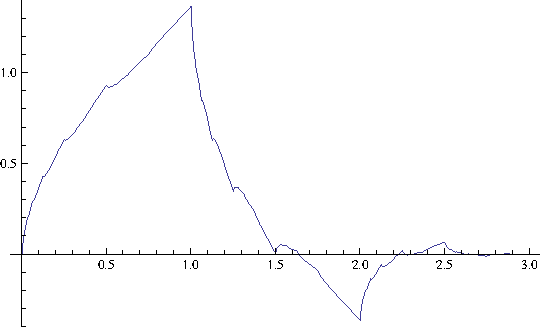
\includegraphics[width=\linewidth]{plaatjes/db2_phi.pdf}
  \end{subfigure}
  \begin{subfigure}{0.48\linewidth}
    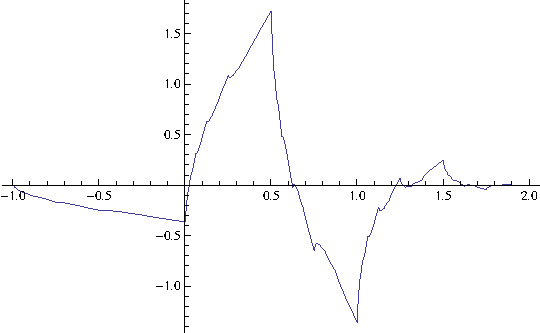
\includegraphics[width=\linewidth]{plaatjes/db2_psi.pdf}
  \end{subfigure}
  \caption{Links: de Daubechies-2 schalingsfunctie. Rechts: de Daubechies-2 waveletfunctie.}
\end{figure}

\section{Fast Wavelet Transform}

Door de recursieve relatie van de ruimtes in \eqref{ruimterec} herhaald toe te passen,
kunnen we de ruimte $V_j$ schrijven in termen van $V_0$ en een scala aan
orthogonaal-complementsruimtes $W_k$, volgens:
\begin{equation}
  \label{ruimte_splitsing}
  V_j = V_k \oplus W_k \oplus \cdots \oplus W_{j-1} = \ldots
  = V_0 \oplus W_0 \oplus \cdots \oplus W_{j-1}.
\end{equation}
We willen een functie $f$ benaderen in de ruimte $V_j$ door $P_{V_j}f$ te schrijven in
de basis van de ruimtes $V_0$ en de verschillende ruimtes $W_k$. Hiervoor dienen we de inproducten
te berekenen van $f$ met de basisvectoren in deze ruimtes.
We onderscheiden dan de \emph{approximatie}-co\"effici\"enten $a_j[n]$ en 
de \emph{detail}-co\"effici\"enten $d_j[n]$, die
$f$ geven als projectie op  respectievelijk $V_j$ en $W_j$.

Het is echter veel rekenwerk om al deze co\"effici\"enten uit te rekenen. 
Dit gebeurt immers door het berekenen van integralen. 
We beperken ons daarom tot het uit rekenen van de co\"effici\"enten op het niveau $j$ 
en proberen vervolgens een recursieve relatie te vinden
om hieruit de approximatie- en detailco\"effici\"enten van het volgende niveau te vinden.

Vanwege de relatie in \eqref{ruimterec} kunnen we de basisfuncties uit de ruimtes $W_{j-1}$,
$V_{j-1}$ schrijven in termen van de basisfuncties van de ruimte $V_j$.
We schrijven daarvoor $\phi_{j-1,n}$ om in termen van de basisfuncties $\phi_{j,k}$ 
en doen dit ook voor $\psi_{j-1,n}$:
\begin{equation}
  \label{phi_rec}
  \phi_{j-1,n} = \sum_{k=-\infty}^{\infty} \inpr{\phi_{j-1,n}}{\phi_{j,k}} \phi_{j,k},
\end{equation}
\begin{equation}
  \label{psi_rec}
  \psi_{j-1,n} = \sum_{k=-\infty}^{\infty} \inpr{\psi_{j-1,n}}{\phi_{j,k}} \phi_{j,k}.
\end{equation}
We rekenen vervolgens de inproducten uit in termen van filterco\"effici\"enten, bekijk:
\eq{
  \inpr{\phi_{j-1,n}}{\phi_{j,k}}
  =& \int_{-\infty}^\infty \sqrt{2^{j-1}}\phi(2^{j-1}t -n)
  \sqrt{2^{j}}\phi^\star(2^j t - k) \d{t}\\
  =& \int_{-\infty}^\infty \tfrac{1}{2^{j-1}} 2^{j-1}
  \sqrt{2} \phi(t') \phi^\star(2t' - k + 2n) \d{t'}\\
  =& \inpr{\phi(t)}{\sqrt{2}\phi(2t-k+2n)} \\
  =& h[k-2n],
}
\eq{
  \inpr{\psi_{j-1,n}}{\phi_{j,k}}
  =& \int_{-\infty}^\infty \sqrt{2^{j-1}}\psi(2^{j-1}t -n)
  \sqrt{2^{j}}\phi^\star(2^j t - k) \d{t}\\
  =& \int_{-\infty}^\infty \tfrac{1}{2^{j-1}} 2^{j-1}
  \sqrt{2} \psi(t') \phi^\star(2t' - k + 2n) \d{t'}\\
  =& \inpr{\psi(t)}{\sqrt{2}\phi(2t-k+2n)} \\
  =& g[k-2n],
}
waarbij we de co\"ordinaattransformatie $t' = 2^{j-1}t - n$ hebben gebruikt.
Door vervolgens aan beide zijden van vergelijkingen \eqref{phi_rec}, \eqref{psi_rec} het
inproduct met $f$ te nemen kunnen we de coe\"ffici\"enten van de resolutie $2^{j-1}$ schrijven
in termen van de co\"effici\"enten op de resolutie $2^j$:
\begin{equation}
  \label{approx_rec}
  a_{j-1}[n] = \inpr{f}{\phi_{j-1,n}}
  = \sum_{k=-\infty}^{\infty} h[k-2n] \inpr{f}{\phi_{j,k}}
  = \sum_{k=-\infty}^\infty h[k-2n] a_{j}[k]
  = (a_j \star \bar h)[2n],
\end{equation}
\begin{equation}
  \label{detail_rec}
  d_{j-1}[n] = \inpr{f}{\psi_{j-1,n}}
  = \sum_{k=-\infty}^{\infty} g[k-2n] \inpr{f}{\phi_{j,k}}
  = \sum_{k=-\infty}^\infty g[k-2n] a_{j}[k]
  = (a_j \star \bar g)[2n],
\end{equation}
waarbij $\bar f: x \mapsto f(-x)$.
De relatie die hier gevonden is geeft aanleiding tot een algoritme.

\begin{algo}[Fast Wavelet Transform]
  Gegeven een rij co\"effici\"enten $a_j\in\R^{2^j}$ defini\"eeren we een recursief
  algoritme $\mathrm{FWT}:\R^{2^j}\to\R^{2^j}$ met een gevalsonderscheid over $j$.\\
  Als $j=0$ dan geldt
  \[
  \mathrm{FWT}(a_j)[n] = a_j[n].
  \]
  Als $j>0$ bereken $a_{j-1}$ en $d_{j-1}$ volgens \eqref{approx_rec}, \eqref{detail_rec}.
  Hiermee berekenen we de $\mathrm{FWT}$ als:
  \begin{equation}
    \label{FWT_cases}
    \mathrm{FWT}(a_j)[n] = \begin{cases}
      \mathrm{FWT}(a_{j-1})[n] & \text{als } n\leq 2^{j-1} \\
      d_{j-1}[n] & \text{als } n>2^{j-1} \end{cases}.
  \end{equation}
\end{algo}
We gaan uit van een eindige filter en beschouwen $V_j$ als een ruimte van functies op een interval in $\R$, 
dan versimpelen de oneindige sommaties in \eqref{approx_rec}, \eqref{detail_rec} tot een eindige som. 

We kunnen nu de transformatie inverteren aan de hand van het volgende algoritme
\begin{algo}[Inverse Fast Wavelet Transform]
  Gegeven een rij co\"effici\"enten $x_j\in\R^{2^j}$ definie\"eren we een recursief
  algoritme $\mathrm{iFWT}:\R^{2^j}\to\R^{2^j}$ met een gevalsonderscheid in $j$.\\
  Als $j=0$ dan geldt
  \[
  \mathrm{iFWT}(x_j)[n] = x_j[n]
  \]
  Als $j>0$, laat $x_{j-1}[n] = x_j[n]$ en $d_{j-1}[n] = x_j[n+2^{j-1}]$ voor $1\leq n\leq 2^{j-1}$. 
  Bereken hiermee $a_{j-1} = iFWT(x_{j-1})$,
  dan geldt
  \begin{equation}
    \label{reconstr_FWT}
    \mathrm{iFWT}(x_j)[n] = (\breve a_{j-1}\star h)[n] + (\breve d_{j-1}\star g)[n],
  \end{equation}
  waarbij $\breve y [2n] = y[n]$ en $\breve y [2n+1] = 0$.
\end{algo}
\begin{stelling}
  De iFWT (links) samengesteld met de FWT geeft de identiteit.
\end{stelling}
\begin{proof}[Bewijs]
  We bekijken de verschillende gevallen. Voor het geval $j=0$ geldt duidelijk dat
  \[
  \mathrm{iFWT}(\mathrm{FWT}(a_0)) = \mathrm{iFWT}(a_0) = a_0.
  \]
  We zullen dus verder moeten bewijzen dat \eqref{reconstr_FWT} een inverse vormt voor
  \eqref{FWT_cases}.
  Schrijf hiervoor de basisfuncties van $V_j$ in termen van de basisfuncties van $V_{j-1}$
  en $W_{j-1}$, ofwel:
  \[
  \phi_{j,n} = \sum_{k=-\infty}^\infty \inpr{\phi_{j,n}}{\phi_{j-1,k}}\phi_{j-1,k}
  + \sum_{-\infty}^\infty \inpr{\phi_{j,n}}{\psi_{j-1,k}}\psi_{j-1,k}.
  \]
  Deze inproducten komen weer overeen met de filterco\"effici\"enten. Nemen we dus aan
  beide zeiden het inproduct dan volgt
  \[
  a_j[n] = \sum_{k=-\infty}^\infty h[n-2k]a_{j-1}[k]
  + \sum_{-\infty}^\infty g[n-2k]d_{j-1}[k].
  \]
  Door in de sommatie de variabele $k$ te vervangen door $k'=2k$ vereenvoudigt dit tot
  \[
  a_j[n] = \sum_{k'=-\infty}^\infty h[n-k']\breve a_{j-1}[k']
  + \sum_{-\infty}^\infty g[n-k']\breve d_{j-1}[k'].
  \]
  Daarmee geeft de iFWT een inverse voor de FWT.
\end{proof}

\section{Analyse van de Wavelettransformatie}
Met de theoretische beschouwing van wavelets en de Fast Wavelet Transform achter de rug, 
zullen we kijken naar practische obstakels.

\subsection{Eindige signalen}
Een van de eerste aannames die we tot nu toe steeds maakten is dat de signalen oneindig lang zijn. 
Wanneer echter de functie $f$ een compacte drager heeft, worden een aantal zaken wat lastiger. 
Neem als eerste aan dat de drager van $f$ binnen $[0,1]$ ligt.
\footnote{Door translatie en dilatie kan elk signaal met compacte basis omgevormd worden tot 
  een signaal met drager binnen $[0,1]$. We verliezen hier dus geen algemeenheid.} 
In dit geval zou het kunnen dat de waveletfuncties met een drager die $t=0$ of $t=1$ doorsnijden, 
niet meer de gewenste eigenschappen hebeben. 
Er zijn in de literatuur oplossingen voor dit probleem gevonden maar hier zullen wij verder niet op in gaan.

Verder namen we ook aan dat de signalen non-discreet zijn. In de praktijk zullen we discrete functies bekijken
die bijvoorbeeld op de resolutie $2^j$ in elk interval een waarde aannemen. We bekijken de multiresolutie
\[
V_0 \subset V_{1} \subset \ldots \subset V_{j}.
\]
We weten nu dat er in $V_j$ een functie $h$ bevat ligt zodat $\inpr{h}{\phi_{j,k}} = f[k]$, deze komt
overeen met onze $f$.
Dit discrete signaal kan dus perfect geschreven worden in de waveletbasis op resolutie $2^{j}$. 
Om deze reden wordt de Fast Wavelet Transform veel gebruikt bij de analyse van discrete signalen.

\subsection{Signaaluitbreiding}
Een probleem waar we in het geval van eindige signalen nog meer mee te maken krijgen is dat de 
algoritme niet goed omgaat met de `randen' van de functie. 
De convolutie heeft ineens informatie nodig die \emph{buiten het definitiegebied} van het signaal ligt. 
Eerder in sectie \ref{signaal} hebben we al gezien hoe signalen naar een tweemacht uitgebreid kunnen worden. 
Precies dezelfde methoden kunnen gebruikt worden om het signaal nog verder uit te breiden.

Om niet te veel tijd te verliezen met het ondersteunen van meerdere mogelijkheden hebben wij er voor gekozen om \emph{periodic padding} op alle signalen toe te passen. 
Dit omdat de zogenaamde \emph{circulaire convolutie} ingebouwd zit in de bibliotheek die wij gebruikt hebben.

\subsection{Complexiteit van de algoritme}
Als de lengte van de filter $h$ gelijk is aan $K$, en de lengte van het originele signaal $a_L$ 
gelijk is aan $N = 2^{L}$,
 kunnen we voor $j \in \{0, \ldots, L\}$ zien dat $a_j$ en $d_j$ beide $2^{j}$ elementen bevatten. 
Vervolgens kunnen $a_{j-1}$ en $d_{j-1}$ gemaakt worden door $2^{j}K$ operaties zodat elke stap van de algoritme 
$2^{j} \cdot K$ operaties kost. 
Daarmee kost het hele algoritme
\[
\sum_{j=0}^L 2^{j} \cdot K = K \sum_{j=0}^L 2^{j} = K \cdot (2^{1+L} - 1) \simeq 2 \cdot K 2^{L} = 2KN
\]
operaties. Dus deze DWT is een $\theta(KN)$ algoritme. 
Ook de complexiteit van de inverse wordt zo van orde $KN$.

\section{Meer dimensies: de Mallatdecompositie}
Met een orthonormale waveletbasis $\{ \psi_{j,n}: (j,n) \in \Z^2\}$ van $L_2(\R)$ volgt een natuurlijke voortzetting
van de waveletfamilie naar twee dimensies door
\[
\{ \psi_{j_1,n_1}(x_1) \psi_{j_2,n_2}(x_2): (j_i,n_i) \in \Z^4 \},
\]
wat een orthonormale basis voor $L_2(\R^2)$ is. 
We zien direct dat we met zulke wavelets op de $x_1$-as met resolutie $2^{j_1}$ kijken 
terwijl de $x_2$-as een resolutie $2^{j_2}$ kent.

Mallat vond dit iets om te vermijden \cite[\S 7.7]{mallat} en legt in zijn analyse dan ook de eis $j_1 = j_2 =: j$ op. 
Wij zullen in het vervolg \'o\'ok kijken naar het zogenaamde Tensorproduct, wat de eis $j_1 = j_2$ \emph{niet} oplegt,
dit volgt in sectie \ref{tensorS}.

In 1 dimensie hebben de notie van `een resolutie' geformaliseerd in het begrip multiresolutie.
De definitie van deze multiresolutie zullen we nu voortzetten naar een meerdimensionaal geval. 
Wanneer we spreken over een separeerbare multiresolutie, bedoelen we een ruimte $V_j^{(2)} := V_j \otimes V_j$,
waarbij $V_j$ tot een \'e\'en-dimensionale multiresolutie behoort.
In \cite[A.5]{mallat} wordt bewezen dat, gegeven een orthonormale basis $\{ \phi_{j,m}: m \in \Z \}$ voor $V_j$, de verzameling
\begin{equation}
  \label{phi_phi_basis}
  \{ \phi^{(2)}_{j,n=(n_1,n_2)} := \phi_{j,n_1} \otimes \phi_{j,n_2}: n \in \Z^2 \}
\end{equation}
een orthonormale basis voor $V_j^{(2)}$ is.

\begin{voorbeeld}
Bekijk weer $V_j$, de ruimte van stuksgewijs constante functies op het interval 
\[
 [2^{-j} m, 2^{-j}(m+1) ) \quad m \in \Z.
\] 
We vinden voor $V_j^{(2)}$ de ruimte van stuksgewijs constante functies op vierkanten van de vorm 
$[2^{-j}n_1, 2^{-j}(n_1+1)) \times [2^{-j}n_2, 2^{-j}(n_2+1))$. 
De tweedimensionale schalingsfunctie wordt nu:
\[
	\phi^{(2)}(x_1,x_2) = \phi(x_1)\phi(x_2) = 
\begin{cases} 1 & \text{ als } x_1 \in [0,1)\text{ en }x_2 \in [0,1) \\ 0 & \text{ anders.} \end{cases}.
\]
\end{voorbeeld}

\subsection{Tweedimensionale Waveletfuncties}
Voor de tweedimensionale ruimtes $V^{(2)}_{j+1}$ die we gevonden hebben willen we nu weer een recursieve
relatie vinden. We weten dat $V_j^{(2)}$ bevat is in $V_{j+1}^{(2)}$, bekijk daarom het orthogonale complement 
$\boldsymbol{U}_j \perp V_j^{(2)}$:
\begin{equation}
  \label{2d_ruimte_rec}
  V_{j+1}^{(2)} =  \boldsymbol{U}_j \oplus V_j^{(2)}
\end{equation}
Om een orthogonale waveletbasis voor $\boldsymbol{U}_j$ te vinden, gaan we als volgt te werk.
Gegeven een waveletbasis voor $V_j$ geinduceerd door de functies $\phi$ en $\psi$, maken we
tweedimensionale wavelets in de ruimte $V_j^{(2)}$ volgens:
\begin{equation}
  \label{psi_k_defs}
  \psi^1(x_1,x_2) = \phi(x_1)\psi(x_2) 
  \quad \psi^2(x_1,x_2) = \psi(x_1) \phi(x_2) 
  \quad \psi^3(x_1,x_2) = \psi(x_1)\psi(x_2).
\end{equation}
Deze functies kunnen we vervolgens schuiven en dilateren. Hiermee verkrijgen we
\begin{equation}
  \label{real_psi_k_defs}
\psi^k_{j,n=(n_1,n_2)}(x_1,x_2) = 2^j \psi^k\left( 2^jx_1 - n_1, 2^j x_2 - n_2 \right)
\end{equation}
en we zullen bewijzen dat deze functies tezamen met $\phi^{(2)}_{0,n}$ een basis vormen voor $L_2(\R)$
\begin{stelling}[{\cite[T7.24]{mallat}}]
  \label{mallatbasis}
  Laat $\phi^{(2)}$ zoals in \eqref{phi_phi_basis}, de $\psi^k$'s zoals in \eqref{real_psi_k_defs} gedefinieerd.
  Dan kunnen we een basis $\boldsymbol{\Psi}_j$ maken voor $\boldsymbol{U}_j$ volgens:
  \[
  \boldsymbol\Psi_j := \{ \psi^1_{j,n}, \psi^2_{j,n}, \psi^3_{j,n}: n \in \Z^2 \}.
  \] 
  Het samennemen van deze bases met een basis voor $V_0^{(2)}$ geeft bovendien 
  \[
  \boldsymbol\Phi := \{ \phi^{(2)}_{0, n}: n \in \Z^2 \} \cup \{ \psi^1_{j,n}, \psi^2_{j,n}, \psi^3_{j,n}: n \in \Z^2, j \in \N_0 \},
  \] 
  wat een basis vormt voor $L_2(\R^2)$.
\end{stelling}
\begin{proof}[Bewijs]
  We schrijven de ruimte $V_{j+1}^{(2)}$ uit als een tensorproduct van ruimtes
  \[
  V_{j+1}^{(2)} = V_{j+1} \otimes V_{j+1}
  \]
  en splitsen de termen, die allen \'e\'en-dimensionale ruimtes zijn, op in de volgende niveau's
  ($V_{j+1} = V_j \oplus W_j$) om te vinden dat:
  \begin{equation*}
  \begin{split}
    V_{j+1} \otimes V_{j+1} =&\, ( V_j \oplus W_j ) \otimes (V_j \oplus W_j ) \\ 
                            =&\, (V_j \otimes V_j) \oplus (V_j \otimes W_j) 
                        \oplus (W_j \otimes V_j) \oplus (W_j \otimes W_j).
  \end{split}
  \end{equation*}
  Gebruik makende van de relatie \eqref{2d_ruimte_rec} leiden we af dat 
  \[
    \boldsymbol{U}_j = (V_j \otimes W_j) \oplus (W_j \otimes V_j) \oplus (W_j \otimes W_j).
  \]
  Omdat de $\psi^k$'s allen tensorproducten zijn van functies in de ruimtes $V_j$ en $W_j$ volgt
  dat $\boldsymbol\Psi_j = \{ \psi^1_{j,n}, \psi^2_{j,n}, \psi^3_{j,n} \largediv  n \in \Z^2 \}$ 
  een basis is voor $\boldsymbol{U}_j$.

  Met de basis van $\boldsymbol{U}_j$ kunnen we vervolgens een basis voor $L_2(\R^2)$ vinden. We schrijven daarvoor
  \[
  L_2(\R^2) = \lim_{j \to \infty} V_j^{(2)} = 
  \lim_{j \to \infty} ( V_0^{(2)} \oplus \boldsymbol{U}_0 \oplus \cdots \oplus \boldsymbol{U}_{j-1} ) = 
   V_0^{(2)} \oplus \left( \bigoplus_{j=0}^\infty \boldsymbol{U}_j \right),
  \]
  zodat
  $\boldsymbol{\Phi} = \{ \phi^{(2)}_{0, n}: n \in \Z^2 \} \cup \{ \psi^1_{j,n}, \psi^2_{j,n}, \psi^3_{j,n}: n \in \Z^2, j \in \N_0 \}$
  een basis is voor $L_2(\R^2)$.
\end{proof}
\begin{gevolg}
We kunnen de laatste paar regels van het bewijs ook gedeeltelijk toepassen door te stoppen bij een ruimte $V_j$.
We vinden dan dat: 
\[
\left\{ \phi^{(2)}_{0, n}: n \in \Z^2 \right\} \cup 
\left\{ \psi^1_{p,n}, \psi^2_{p,n}, \psi^3_{p,n}: n \in \Z^2, 
p \in \{0, \ldots, j \}  \right\}
\]
een orthonormale basis voor $V_j^{(2)}$ is.
\end{gevolg}

Bovenstaande basis bevat dus het tensorproduct van twee schalingsfuncties op \'e\'en niveau 
en verder combinaties van schalings- en waveletfuncties van dezelfde resolutie op alle niveaus. 
Net zoals in het eendimensionale geval kunnen we met deze basis een algoritme formuleren.

\subsection{Naar een tweedimensionaal algoritme}
Nu we volgens \eqref{2d_ruimte_rec} een relatie hebben gevonden tussen de ruimtes, namelijk
\begin{equation}
  \label{2d_ruimte_decomp}
V_{j+1}^{(2)} = (V_j\otimes W_j) \oplus (W_j\otimes V_j) \oplus
(W_j\otimes W_j) \oplus (V_j\otimes V_j),
\end{equation}
kunnen we het eendimensionale algoritme uitbreiden naar twee dimensies.
Hiervoor kijken we wederom naar de inproducten van een functie $f$ met onze basisfuncties.
We defini\"eren daarvoor weer de \emph{approximatie}-co\"effici\"ent en drietallen
van \emph{detail}-co\"effici\"enten volgens:
\[
a_j[n] := \langle f, \phi^{(2)}_{j,n} \rangle, 
\quad d^p_j[n] := \langle f, \psi^p_{j,n} \rangle \text{voor} \quad p \in \{1,2,3\}.
\]
We zullen in het bijzonder de basis-functies op het niveau $j$ kunnen ontbinden 
door gebruik te maken van $\eqref{phi_phi_basis}$:
\begin{equation}
  \label{phi_phi_som}
  \phi^{(2)}_{j,(n_1,n_2)} = \sum_{k_1=-\infty}^\infty \sum_{k_2=-\infty}^\infty
  \inpr{\phi_{j,n_1}\otimes\phi_{j,n_2}}{\phi_{j+1,k_1}\otimes\phi_{j+1,k_2}}
  \phi^{(2)}_{j+1,(k_1,k_2)}
\end{equation}
\begin{equation}
  \label{psi_k_som}
  \psi^{p}_{j,(n_1,n_2)} = \sum_{k_1=-\infty}^\infty \sum_{k_2=-\infty}^\infty
  \inpr{\psi^p_{j,(n_1,n_2)}}{\phi_{j+1,k_1}\otimes\phi_{j+1,k_2}}
  \phi^{(2)}_{j+1,(k_1,k_2)}
\end{equation}
We maken nu gebruik van \cite[\S 3.4]{weidmann} om het inproduct horende bij het tensorproduct
van twee \emph{Hilbertruimten} uit te schrijven als:
\[
\inpr{a\otimes b}{c\otimes d} = \inpr{a}{c}\cdot \inpr{b}{d},
\]
waarbij de inproducten behoren bij de respectievelijke ruimtes.
Dit versimpelt de inproducten die we zoeken volgens:
\[
\inpr{\phi_{j,n_1}\otimes\phi_{j,n_2}}{\phi_{j+1,k_1}\otimes\phi_{j+1,k_2}}
=\inpr{\phi_{j,n_1}}{\phi_{j+1,k_1}}\inpr{\phi_{j,n_2}}{\phi_{j+1,k_2}}
=h[k_1-2n_1]\cdot h[k_2-2n_2],
\]
waarbij we de filterrelatie voor \'e\'en dimensie toepassen. We kunnen dit nog een
stuk verbeteren door het product $h[\_]\cdot h[\_]$ om te schrijven naar een tensorproduct,
namelijk:
\[
(h\otimes h)(x_1,x_2) =  h[x_1]\cdot h[x_2]
\]
Deze stappen kunnen met hetzelfde argument toegepast worden op de $\psi^k$'s.
We verkrijgen dan met een blik op de definities in $\eqref{psi_k_defs}$ de vergelijkingen:
\[
\inpr{\psi^1_{j,(n_1,n_2)}}{\phi^{(2)}_{j+1,(k_1,k_2)}} = (h\otimes g) [k_1-2n_1,k_2-2n_2]
\]
\[
\inpr{\psi^2_{j,(n_1,n_2)}}{\phi^{(2)}_{j+1,(k_1,k_2)}} = (g\otimes h) [k_1-2n_1,k_2-2n_2]
\]
\[
\inpr{\psi^3_{j,(n_1,n_2)}}{\phi^{(2)}_{j+1,(k_1,k_2)}} = (g\otimes g) [k_1-2n_1,k_2-2n_2]
\]
Vervolgens richten we ons weer op de approximatie- en detail-co\"effici\"enten door
aan beide zijden van de vergelijkingen $\eqref{phi_phi_som}$, $\eqref{psi_k_som}$ het inproduct
met $f$ te nemen. We kunnen dit aan de hand van onze nieuwe 2-dimensionale filters
opschrijven met een convolutie in twee dimensies:
\begin{eqnarray}
  \label{2d_coef_rec}
  a_{j}[n_1,n_2] =& (a_{j+1} \star (\bar{h} \otimes \bar{h}))[2n_1,2n_2] \\
  d^1_{j}[n_1,n_2] =&( a_{j+1} \star (\bar{h} \otimes \bar{g}))[2n_1,2n_2] \\
  d^2_{j}[n_1,n_2] =& (a_{j+1} \star (\bar{g} \otimes \bar{h}))[2n_1,2n_2] \\
  \label{2d_coef_rec_last}
  d^3_{j}[n_1,n_2] =& (a_{j+1} \star (\bar{g} \otimes \bar{g}))[2n_1,2n_2].
\end{eqnarray}
waarbij de tweedimensionale convolutie gegeven wordt door
\[
(x \star y)[n_1,n_2] := \sum_{p_1=-\infty}^\infty \sum_{p_2 = -\infty}^\infty
x[n_1 - p_1,n_2 - p_2] \cdot y[n_1-p_1, n_2 - p_2].
\]

\begin{algo}[Tweedimensionale Fast Wavelet Transform]
  Gegeven een matrix van co\"effici\"enten $a_j\in\R^{2^j}\times\R^{2^j}$, definie\"eren
  we een algoritme \mbox{$\mathrm{FWT}_2:\R^{2^j}\times\R^{2^j}\to\R^{2^j}\times\R^{2^j}$}.\\
  Als $j=0$ dan geldt
  \[
  \mathrm{FWT}_2(a_j)[n_1,n_2] = a_j[n_1,n_2]
  \]
  Als $j>0$ bereken $a_{j-1}$,$d^1_{j-1}$,$d^2_{j-1}$ en $d^3_{j-1}$ uit $a_{j}$
  volgens $(\eqref{2d_coef_rec}-\eqref{2d_coef_rec_last})$.
  Dan geldt
  \begin{equation}
    \label{FWTd_def}
  \mathrm{FWT}_2(a_j)[n_1,n_2] = \begin{cases}
    \mathrm{FWT}_2(a_{j-1})[n_1,n_2] & \text{als } n_1 \leq 2^{j-1} \text{ en } n_2 \leq 2^{j-1}\\
    d^1_{j-1}[n_1,n_2]
    & \text{als } n_1\leq 2^{j-1} \text{ en } n_2>2^{j-1} \\
    d^2_{j-1}[n_1,n_2]
    & \text{als } n_1>2^{j-1} \text{ en } n_2\leq 2^{j-1} \\
    d^3_{j-1}[n_1,n_2] & \text{als } n_1>2^{j-1} \text{ en } n_2>2^{j-1} \end{cases}
  \end{equation}
\end{algo}
Van dit tweedimensionale algoritme kunnen nu ook de inverse algoritme bepalen, analoog aan het eendimensionale geval.
\begin{algo}[Inverse Tweedimensionale Fast Wavelet Transform]
  Gegeven een matrix van  co\"effici\"enten $x_j\in\R^{2^j}\times\R^{2^j}$, defini\"eeren we hierop het
  algoritme \mbox{$\mathrm{iFWT}_2:\R^{2^j}\times\R^{2^j}\to\R^{2^j}\times\R^{2^j}$}.\\
  Als $j=0$ dan geldt
  \[
  \mathrm{iFWT}_2(x_j)[n_1,n_2] = x_j[n_1,n_2]
  \]
  Als $j>0$, splits dan $x_j$ in zijn vier kwadranten; laat voor $k_1,k_2\in \{1,\ldots,2^{j-1}\}$
  \begin{eqnarray*}
    y_{j-1}[k_1,k_2]   =& x_j[k_1,k_2] \\
    d^1_{j-1}[k_1,k_2] =& x_j[k_1,k_2+2^{j-1}] \\
    d^2_{j-1}[k_1,k_2] =& x_j[k_1+2^{j-1},k_2] \\
    d^3_{j-1}[k_1,k_2] =& x_j[k_1+2^{j-1},k_2+2^{j-1}]
  \end{eqnarray*}
  Bereken hiermee vervolgens $a_{j-1} = \mathrm{iFWT}_2(y_{j-1})$,
  dan geldt
  \begin{equation}
    \label{iFWTd_def}
    \begin{split}
      \mathrm{iFWT}_2(a_j)[n_1,n_2] =&\, \breve{a}_{j-1} \star (h \otimes h)[n_1,n_2] 
      + \breve{d}_{j-1}^1 \star (h \otimes g)[n_1,n_2] \\
      +&\, \breve{d}_{j-1}^2 \star (g \otimes h)[n_1,n_2] 
      + \breve{d}_{j-1}^3 \star (g \otimes g)[n_1,n_2]
    \end{split}
  \end{equation}
  waarbij 
  \[
  \breve y [n_1,n_2] = \begin{cases} 
    y[n_1/2,n_2/2] & \text{als } 2|n_1 \text{ en } 2|n_2 \\ 
    0 &\text{anders.}\end{cases}
  \]
\end{algo}
\begin{stelling}
  De $\mathrm{iFWT}_2$ (links) samengesteld met de $\mathrm{FWT}_2$ geeft de identiteit.
\end{stelling}
\begin{proof}[Bewijs]
  We bekijken de verschillende gevallen. Voor het geval $j=0$ geldt duidelijk dat
  \[
  \mathrm{iFWT}_2(\mathrm{FWT}_2(a_0)) = \mathrm{iFWT}_2(a_0) = a_0.
  \]
  Voor het geval $j>0$ merken we op dat wanneer de $\mathrm{iFWT}_2$ werkt voor $j'<j$ de co\"effici\"enten-matrices
  $a,d^1,d^2,d^3$ precies zijn wat de $\mathrm{FWT}_2$ zou geven op dit niveau. 
  We zullen dus verder moeten bewijzen dat \eqref{iFWTd_def} een inverse vormt voor
  \eqref{FWTd_def}.
  Schrijf hiervoor de basisfuncties van $V^{(2)}_j$ in termen van de basisfuncties van
  de tensorproductenruimte van $V_j$ en $W_j$ zoals in \eqref{2d_ruimte_decomp}:
  \begin{equation*}
    \begin{split}
      \phi_{j,(n_1,n_2)} = 
      \sum_{k_1=-\infty}^\infty\sum_{k_2=-\infty}^\infty 
      \inpr{\phi^{(2)}_{j,(n_1,n_2)}}{\phi^{(2)}_{j-1,(k_1,k_2)}} \phi^{(2)}_{j-1,(k_1,k_2)} \\
      + \sum_{k_1=-\infty}^\infty\sum_{k_2=-\infty}^\infty 
      \inpr{\phi^{(2)}_{j,(n_1,n_2)}}{\psi^1_{j-1,(k_1,k_2)}} \psi^1_{j-1,(k_1,k_2)} \\
      + \sum_{k_1=-\infty}^\infty\sum_{k_2=-\infty}^\infty 
      \inpr{\phi^{(2)}_{j,(n_1,n_2)}}{\psi^2_{j-1,(k_1,k_2)}} \psi^2_{j-1,(k_1,k_2)} \\
      + \sum_{k_1=-\infty}^\infty\sum_{k_2=-\infty}^\infty 
      \inpr{\phi^{(2)}_{j,(n_1,n_2)}}{\psi^3_{j-1,(k_1,k_2)}} \psi^3_{j-1,(k_1,k_2)}.
      \end{split}
  \end{equation*}
  Deze inproducten tussen basisfuncties komen weer overeen met de filterco\"effici\"enten. Nemen we dus aan
  beide zeiden het inproduct met $f$ dan volgt de vergelijking voor de approximatie-co\"effici\"enten
  \begin{equation*}
    \begin{split}
      a_{j}[n_1,n_2] = 
      \sum_{k_1=-\infty}^\infty\sum_{k_2=-\infty}^\infty 
      (h\otimes h)[n_1-2k_1,n_2-2k_2] a_{j-1}[k_1,k_2] \\
      + \sum_{k_1=-\infty}^\infty\sum_{k_2=-\infty}^\infty 
      (h\otimes g)[n_1-2k_1,n_2-2k_2] d^1_{j-1}[k_1,k_2] \\
      + \sum_{k_1=-\infty}^\infty\sum_{k_2=-\infty}^\infty 
      (g\otimes h)[n_1-2k_1,n_2-2k_2] d^2_{j-1}[k_1,k_2] \\
      + \sum_{k_1=-\infty}^\infty\sum_{k_2=-\infty}^\infty 
      (g\otimes g)[n_1-2k_1,n_2-2k_2] d^3_{j-1}[k_1,k_2].
      \end{split}
  \end{equation*}
  Door in de sommatie de variabelen $k_1,k_2$ te vervangen door $k_1'=2k_1$ respectievelijk $k_2'=2k_2$ 
  vereenvoudigt dit tot
  \begin{equation*}
    \begin{split}
      a_{j}[n_1,n_2] = 
      \sum_{k_1'=-\infty}^\infty\sum_{k_2'=-\infty}^\infty 
      (h\otimes h)[n_1-k_1',n_2-k_2'] \breve a_{j-1}[k_1',k_2'] \\
      + \sum_{k_1'=-\infty}^\infty\sum_{k_2'=-\infty}^\infty 
      (h\otimes g)[n_1-k_1',n_2-k_2'] \breve d^1_{j-1}[k_1',k_2'] \\
      + \sum_{k_1'=-\infty}^\infty\sum_{k_2'=-\infty}^\infty 
      (g\otimes h)[n_1-k_1',n_2-k_2'] \breve d^2_{j-1}[k_1',k_2'] \\
      + \sum_{k_1'=-\infty}^\infty\sum_{k_2'=-\infty}^\infty 
      (g\otimes g)[n_1-k_1',n_2-k_2'] \breve d^3_{j-1}[k_1',k_2'],
      \end{split}
  \end{equation*}
  wat precies de convolutie in \eqref{iFWTd_def} is. Daarmee geeft de iFWT een inverse voor de FWT.
\end{proof}

\subsection{Meer dan twee dimensies}
\label{mallat_md}
De Mallatdecompositie is op een natuurlijke manier voort te zetten naar meerdimensionale signalen.
De precieze definitie is notationeel nogal ingewikkeld en laten we hier daarom achterwege.
Informeel geldt dat we een $m$-dimensionale ruimte $V_{j}^{(m)}$ 
weer kunnen schrijven zoals \eqref{2d_ruimte_decomp}
waarbij we dit maal het tensorproduct nemen van $m$ factoren, $V_{j-1}$ en $W_{j-1}$.
De basisfuncties van deze ruimtes zijn vervolgens de tensorproducten van $m$ 
factoren die ofwel $\phi$ of $\psi$ zijn.
Vervolgens kan het algoritme verder doorgezet worden naar de ruimte $V_{j-1}^{(m)}$.
In termen van algoritmen vertaalt dit alles naar een $m$ dimensionale convolutie van $a_j$ met 
filters die het tensorproduct zijn van $m$ factoren $h$ of $g$.
\begin{voorbeeld}
  In drie dimensies maken we een Mallat-decompositie van de ruimte $V_{j+1}^{(3)}$ door:
  \[
  \begin{split}
    V_{j+1}^{(3)} = V_{j}^{(3)} \oplus& \left (V_j^{(2)} \otimes W_j \right) 
                              \oplus \left (V_j\otimes W_j \otimes V_j \right) 
                              \oplus \left (W_j\otimes V_j^{(2)} \right)\\ 
                              \oplus& \left (V_j\otimes W_j^{(2)} \right)  
                              \oplus \left (W_j\otimes V_j \otimes W_j \right) 
                              \oplus \left (W_j^{(2)} \otimes V_j \right) 
                              \oplus W_j^{(3)}
  \end{split}
  \]
  De basisfuncties en filters die hier bijhoren zijn analoog aan de bijbehorende ruimtes.
  Deze filters kunnen we vervolgens toepassen op bijvoorbeeld filmmateriaal.
\end{voorbeeld}

\subsection{Eindige signalen in $n$ dimensies}
De notie van eindige signalen is al eerder langsgekomen. We bekijken functies met een compacte drager $[0,1]$. 
Het gevolg hiervan is dat de complete waveletbasis teveel elementen bevat. 
Alleen wavelets waarvan de drager het interval doorsnijdt, zijn voor ons interessant. 
Wanneer we meer dimensies bekijken, praten we over een $n$-dimensionaal eenheidsinterval $[0,1]^n =: \Box$. 
Wederom zijn alleen de functies van belang wiens drager $\Box$ doorsnijdt.

\section{Tensorproduct}
\label{tensorS}

Herinner dat we voor de Mallat-decompositie gebruik maakte van de gelijkheid:
\[
V_{j}^{(2)} = (V_{j-1}\otimes W_{j-1}) \oplus (W_{j-1}\otimes V_{j-1}) \oplus
(W_{j-1}\otimes W_{j-1}) \oplus (V^{(2)}_{j-1})
\]
Door dit herhaald toe te passen kregen we een basis van de vorm:
\[
\{\phi^{(2)}_{0,(n_11,n_2)}\largediv n_1,n_2\in\Z\}\cup
\{\psi^k_{j,(n_1,n_2)} \largediv k=1,2,3\quad j\in \N_0 \quad n_1,n_2\in\Z\}
\]
We zullen echter zien dat er ook een andere manier is om deze ruimte te decomposeren.
Bedenk dat we in 1 dimensie de decompositie zoals in \eqref{ruimte_splitsing} gebruiken, namelijk:
\[
V_j = V_0 \oplus W_0 \oplus \cdots \oplus W_{j-1}
\]
Daarmee schrijven we de ruimte $V^{(2)}_j$ als het tensorproduct van $V_j$ met zichzelf:
\[
V^{(2)}_j = V_j\otimes V_j = (V_0\oplus W_0\oplus\cdots W_{j-1})\otimes(V_0\oplus W_0\oplus\cdots W_{j-1})
\]
Dit geeft aanleiding tot een nieuwe basis, namelijk het tensorproduct van de basis van $V_j$ met zichzelf,
we duiden deze basis dan ook aan als de \emph{Tensorbasis}~\footnote{In de literatuur wordt de Mallatdecompositie ook regelmatig een tensorproduct genoemd. 
De verwarring ontstaat hier doordat in de Mallatbasis de basisfuncties ook tensorproducten zijn van wavelet- 
en schalingsfuncties. We doelen echter in onze naamgeving op \emph{het tensorproduct van twee bases}.}.
Schrijf namelijk \mbox{$A^2 = \{a\otimes b \largediv a,b\in A\}$} voor het \emph{Tensorproduct} van een basis met zichzelf,
dan krijgen we:
\begin{equation}
  \label{tensor_basis_def}
  \begin{split}
    \boldsymbol\Phi_T :=& (\{\phi_{0,n}\largediv n\in\Z\}\cup \{\psi_{j,n}\largediv j\in\N_0\quad n\in\Z\})^2\\
                        =& \{\phi_{0,n_1}\otimes\phi_{0,n_2}\largediv n_1,n_2\in\Z\} 
                        \cup \{\phi_{0,n_1}\otimes\psi_{j,n_2}\largediv j\in\N_0\quad n_1,n_2\in\Z\} \\    
                         & \cup \{\psi_{j,n_1}\otimes\phi_{0,n_2}\largediv j\in\N_0\quad n_1,n_2\in\Z\} \\
                         & \cup \{\psi_{j_1,n_1}\otimes\psi_{j_2,n_2}\largediv j_1,j_2\in\N_0\quad n_1,n_2\in\Z\}.
  \end{split}
\end{equation}

Een karakteristiek van de Mallatbasis is dat deze $\psi \otimes \psi$ functies bevat van enkel dezelfde schaal,
terwijl we bij de Tensorbasis te maken hebben met $j_1$ en $j_2$ die ongelijk aan elkaar zijn.
De Mallatbasis moest door deze eis aangevuld worden met functies van de vorm $\phi\otimes\psi$ en $\psi\otimes\phi$.
Dit is bij de Tensorbasis niet meer aan de orde (met uitzondering van enkele samenstellingen van $\phi_0$ met $\psi_j$'s)

Met deze theoretische kennis willen we een algoritme bedenken dat een tweedimensionaal signaal schrijft 
in termen van de Tensorbasis. We zullen zien dat dit neerkomt op het uitvoeren van FWT op alle rijen en 
kolommen van de ingangssignaal, die we voorstellen als een matrix.

\begin{algo}[Tweedimensionale Tensor Fast Wavelet Transform]
Gegeven een ingangssignaal $a_j\in\R^{2^j}\times\R^{2^j}$, defini\"eren we een  algoritme 
\mbox{$\mathrm{TFWT}_2:\R^{2^j}\times\R^{2^j}\to \R^{2^j}\times\R^{2^j}$} als volgt.\\
Bereken $\tilde a_j$ zo dat geldt:
\[
\tilde a_j[n_1,n_2] = \mathrm{FWT}(a_j\largediv_{x_1=n_1})[n_2] 
\]
Dan wordt de $\mathrm{TFWT}_2$ gegeven door:
\[
\mathrm{TFWT}_2(a_j)[n_1,n_2] = \mathrm{FWT}(\tilde a_j\largediv_{x_2=n_2})[n_1]
\] 
\end{algo}

We zullen aantonen dat de $\mathrm{TFWT}_2$ ook inderdaad een decompositie geeft in termen van de Tensorbasis.
We zijn namelijk op zoek naar een matrix van de vorm:
\begin{equation}
\label{TFWT_mat}
\begin{bmatrix}
\inpr{f}{\phi_0\otimes\phi_0}     & \inpr{f}{\phi_0\otimes\psi_0}     & \cdots & \inpr{f}{\phi_0\otimes\psi_j} \\
\inpr{f}{\psi_0\otimes\phi_0}     & \inpr{f}{\psi_0\otimes\psi_0}     & \cdots & \inpr{f}{\psi_0\otimes\psi_j} \\ 
           \vdots                 &         \vdots                    & \ddots &                \vdots  \\ 
\inpr{f}{\psi_j\otimes\phi_0} & \inpr{f}{\psi_j\otimes\psi_0} 
& \cdots & \inpr{f}{\psi_j\otimes\psi_j} \\
\end{bmatrix}
\end{equation}
We weten dat wanneer we de FWT nemen in \'e\'en co\"ordinaat door de andere co\"ordinaat vast te nemen,
 dit ons voor elke vaste waarde een vector geeft volgens:
\[
y \mapsto
\begin{bmatrix}
\inpr{f\largediv_{x_2=y}}{\phi_0} & 
\inpr{f\largediv_{x_2=y}}{\psi_0} & \cdots & 
\inpr{f\largediv_{x_2=y}}{\psi_j}
\end{bmatrix}
\]
Hieruit kunnen we ook een vector van functies maken door de rol van functie en matrix-index om te wisselen:
\[
\begin{bmatrix}
y \mapsto \inpr{f\largediv_{x_2=y}}{\phi_0} & 
y \mapsto \inpr{f\largediv_{x_2=y}}{\psi_0} & \cdots & 
y \mapsto \inpr{f\largediv_{x_2=y}}{\psi_j}
\end{bmatrix}
\]
Wanneer we vervolgens voor elke functie in deze vector de FWT bereken zullen we weer een vector inproducten krijgen
voor elke co\"ordinaat in de originele vector, schrijf deze vector van vectoren (equivalent met een matrix) uit als 
$M[k_1,k_2]$,
\footnote{Hier wordt het inproduct met $\phi_0$ weggelaten om de schrijfwijze te verduidelijken. We zien
dan $\phi_0$ als een $\psi_k$ met een speciale index $k$.}
dan volgt:
\[
M[k_1,k_2] = \inpr{y\mapsto \inpr{f\largediv_{x_2=y}}{\psi_{k_1}}}{\psi_{k_2}}
\]
We kunnen dit omschrijven door de definitie van het inproduct op functieruimten toe te passen:
\[
\inpr{y\mapsto \inpr{f\largediv_{x_2=y}}{a}}{b} = 
\int_{-\infty}^\infty\int_{-\infty}^\infty f(x_1,x_2) \cdot a(x_1) \d{x_1} \cdot b(x_2) \d{x_2} = \inpr{f}{a\otimes b} 
\]
Waardoor de matrix $M$ identiek is aan \eqref{TFWT_mat}. 

Het vinden van een inverse voor dit algoritme is hiermee ook triviaal, de iFWT geeft samengesteld met de FWT
immers de identiteit, zodat het toepassen op kolommen en rijen van de iFWT de $\mathrm{TFWT}_2$ inverteert.

\subsection{Meer dan twee dimensies}
\label{tensor_md}
Er is een natuurlijke voortzetting van het Tensorproduct naar meerdimensionale signalen.
Dit doen we door voor bijvoorbeeld  $V^{(m)}_j$ de basis te kiezen die voortkomt uit
een tensorproduct van $m$ maal de basis van $V_j$.
Vervolgens is de algoritme te veralgemeniseren naar een algoritme dat over elke co\"ordinaat de FWT 
uitvoert, met bijbehorende inverse.

Omdat de stap in complexiteit van de notatie vele male groter is dan de benodigde denkstap laten we hier een rigoreuze
behandeling van de meerdimensionale Tensor Fast Wavelet Transform achterwege.

\subsection{Mengvormen van Tensor en Mallat}
Zoals uitgelegd in de secties \ref{tensor_md} en \ref{mallat_md} kunnen zowel de Mallatdecompositie als
het Tensorproduct toegepast worden op $3$ of meer dimensies. We zullen beargumenteren dat de beide
vormen ook naar eigen inzicht gemengd kunnen worden. We schrijven daarvoor de $m$-dimensionale 
ruimte $V_j^{(m)}$ op als een tensorproduct:
\begin{equation*}
\begin{array}{ccccccc}
  V_j^{(m)} &=& V_j^{(k-1)} &\otimes&              V_j                     &\otimes& V_j^{(m-k)} \\
            &=& V_j^{(k-1)} &\otimes& (V_0 \otimes \cdots \otimes W_{j-1}) &\otimes& V_j^{(m-k)}
\end{array}
\end{equation*}
Hier zien we dat de $k$-de term $V_j$ uitgeschreven is volgens de gewone $FWT$
decompositie. Het staat ons nu vrij om de termen $V_j^{(k-1)}$ en $V_j^{m-k}$ te ontbinden
op een andere manier. De gebruikte algoritmes volgen analoog aan de implementatie van het Tensorproduct
en de Mallatdecompositie door co\"ordinaten vast te houden.\footnote{De notatie voor de mengvorm en de specifieke bewijzen laten we achterwege. Deze leiden teveel af van het doel van het project.}

\begin{voorbeeld}
We kunnen in 3 dimensies een Tensor-Mallat mengvorm maken:
\begin{equation}
\label{3d_mengvorm}
\begin{split}
V_j^{(3)} = &
\left (V^{(2)}_{j-1} 
\oplus (W_{j-1}\otimes V_{j-1}) 
\oplus (V_{j-1}\otimes W_{j-1}) 
\oplus (W_{j-1}\otimes W_{j-1}) \right ) \\
&\otimes (V_0\oplus\cdots\oplus W_{j-1})
\end{split}
\end{equation}
Hier is de eerste term ontbonden volgens de Mallatdecompositie en hebben we met het Tensorproduct
een normale FWT decompositie hier recht op gezet.
\end{voorbeeld}
\begin{gevolg}
Wanneer we in \ref{3d_mengvorm} de eerste term opvatten als een ruimte van afbeeldingen op een bepaald moment en
de tweede term als de tijdruimte die het verloop van een afbeelding geeft, dan kunnen we deze
decompositie toepassen op videomateriaal. 
\end{gevolg}

\section{Analyse van de fout van beide decomposities}
\label{daling_wavelet}

Bij compressie is men op zoek naar een manier om stukjes data weg te kunnen gooien of te schrijven op zo'n manier dat het minder ruimte inneemt. Wij zijn in het bijzonder ge\"interesseerd in \emph{hoe dichtbij} we bij perfecte reconstructie zitten wanneer we een vooraf bepaald hoeveelheid data opslaan. Er is al uitgebreid onderzoek gedaan naar hoe dit werkt bij de waveletbasis en een aantal resultaten hiervan zullen we opnemen in ons verslag.

Laat $f$ een functie in $L_2(\Box)$ met aftelbare orthonormale basis $\mathcal{B} = \{ g_m \}$. Dan valt $f$ in deze basis te schrijven als (zie Lemma \ref{parseval})
\begin{equation}
\label{linfout}
f = \sum_{m = 0}^\infty \langle f, g_m \rangle g_m.
\end{equation}

Wanneer we niet de hele basis bekijken, maar slechts een $N$ aantal elementen pakken, 
krijgen we een verzameling $\mathcal{B}_N \subset \mathcal{B}$ zodat
\[
f|_{\mathcal{B}_N} := \sum_{g_m \in \mathcal{B}} \langle f, g_m \rangle g_m.
\]
In het bijzonder zijn we op zoek naar de \emph{fout} van de reconstructie $\| f - f|_{\mathcal{B}_N} \|$:
\[
\| f - f|_{\mathcal{B}_N} \|^2 
= \left\| \sum_{g_m \in \mathcal{B}} \langle f, g_m \rangle g_m - 
\sum_{g_m\in\mathcal{B}_N} \langle f, g_m \rangle g_m \right\|^2 
= \left\| \sum_{g_m\in \mathcal{B}\backslash\mathcal{B}_N} \langle f, g_m \rangle g_m \right\|^2 
= \sum_{g_m\in \mathcal{B}\backslash\mathcal{B}_N} | \langle f, g_m \rangle |^2.
\]
Duidelijk moge zijn dat voor $N \to \infty$, $\| f - f|_{\mathcal{B}_N} \|^2 \to 0$.

\begin{definitie}[Sobolevruimte]
Een Sobolevruimte $H^p(\Omega)$ over $\Omega \subset \R$ is de verzameling van alle functies $u \in L_2(\Omega)$ waarvoor geldt dat
\[
	\frac{\partial^k u}{\partial x^k} \in L_2(\Omega), k \leq p.
\]

De norm op $H^p$ die hierbij hoort is gedefini\"eerd als
\[
	\| u \|_{H^p(\Omega)} := \sum_{k \leq p} \left\| \frac{\partial^k u}{\partial x^k} \right\|_{L_2(\Omega)}.
\]

In $n$ dimensies:
\[
	H^{(p_1,p_2,\ldots,p_n)}(\Box) := \bigotimes_{k=1}^n H^{p_k}([0,1]).
\]
\end{definitie}

\subsection{Fout van de Mallatdecompositie}
Wij zijn op het ge\"interesseerd in de Mallat-waveletbasis $\boldsymbol\Phi$ die we vonden in stelling \ref{mallatbasis}.Deze is duidelijk aftelbaar, dus we kunnen \eqref{linfout} gebruiken. 

Defini\"eer $J_M := \{ l \in \N^n: \| l \|_\infty \leq M \}$. Laat $\boldsymbol\Phi_M := \{ \boldsymbol{\psi}_{\boldsymbol{\lambda}} \in \boldsymbol\Phi: |\boldsymbol\lambda| \in J_M \}$ met \mbox{$|\boldsymbol\lambda| = (|\lambda_1|, \ldots, |\lambda_n|)$} de verzameling basisfuncties tot een niveau $M$.

\begin{stelling}[Fout van Mallatdecompositie]
\label{thm:foutmallat}
Wanneer $f \in H^{(p,\ldots,p)}(\Box)$, zal de fout \mbox{$\| f - f|_{\boldsymbol\Phi_M} \|$} bij een Mallatdecompositie met de basisfuncties tot niveau $M$ precies $\theta(N^{-\tfrac p{2n}})$ zijn, met \mbox{$N := \# \boldsymbol\Phi_M$} het aantal basisfuncties tot niveau $M$.
\end{stelling}
\begin{proof}

  We maken gebruik van de zogenaamde Jacksonongelijkheid \cite{jackson} die zegt dat, gegeven de ruimte $\mathbb{P}_{p-1}$ van polynomen van orde $p-1$, geldt: 
  \[
  \inf_{q \in \mathbb{P}_{p-1}} ||f - q||_{L_2(\Box)} \simeq 2^{-jp} ||f||_{H^{(p,\ldots,p)}(\Box)}
  \]
  wanneer $f \in H^{(p,\ldots,p)}(\Box)$.

  Voor elke dimensie zitten er $\theta(2^M)$ basisfuncties in $\{ \psi_\lambda: |\lambda| \leq M \}$. Er zijn $n$ dimensies dus $2^{Mn} = N$ basisfuncties in totaal. Bekijk de fout:
  \[
  \left\| f - f|_{\boldsymbol\Phi_M} \right\|^2_{L_2(\Box)} 
  = \sum_{{\boldsymbol\psi} \in \boldsymbol\Phi \setminus \boldsymbol\Phi_M} | \langle f, \boldsymbol\psi \rangle |^2 
  \simeq \sum_{|\boldsymbol\lambda| > M} 2^{-|\boldsymbol\lambda|p} \simeq 2^{-Mp},
  \]
  waarbij het laatste gelijkheidsteken voortkomt uit de relatie
  \[
  \sum_{k=M+1}^\infty 2^{- kp} = \frac{2^{-Mp}}{2^p-1}
  \]
  en de notie dat $p$ constant is voor een keuze van de wavelet. 
  De fout is nu $2^{-Mp/2}$. Omschrijven geeft dat dit overeenkomt met een fout van $N^{-\frac p {2n}}$.
\end{proof}

\subsection{Fout van het Tensorproduct}
We bekijken een aftelbare basis van $L_2(\Box)$. In 1 dimensie wordt deze basis gevonden door $\{ \psi_\lambda: \lambda \in \nabla \}$, waarbij $\nabla$ precies de indexverzameling van deze basis is.

Volgens \cite[L3.1.7]{tammo} is 
\[ 
  \boldsymbol\Phi_T = \Phi \otimes \cdots \otimes \Phi = \{ \boldsymbol{\psi_\lambda} := \psi_{\lambda_1} \otimes \cdots \otimes \psi_{\lambda_n}: \lambda_i \in \nabla \}
\]
met $\boldsymbol\lambda := (\lambda_1, \ldots, \lambda_n) \in \boldsymbol{\nabla} := \nabla^n$ een orthogonale basis voor $L_2(\Box)$.

Laat vervolgens $I_M := \{ l \in \N^n_0: ||l||_1 \leq M \}$ en maak de \emph{sparse grid index set} \mbox{$\boldsymbol{\nabla}_M := \{ \boldsymbol{(j,n)} \in \boldsymbol{\nabla}: \boldsymbol{j} \in I_M \}$}.

We zullen nu een aantal lemma's enumereren die we willen gebruiken om de fout af te schatten. De bewijzen hiervoor
staan in \cite{tammo} en zullen we niet verder behandelen.
\begin{lemm}{\cite[P3.2.3]{tammo}}
  \label{en_daarom_jongens_en_meisjes}
  Voor $f \in H^{(p,\ldots,p)}(\Box)$ geldt dat de fout van de benadering op basis van de sparse grid index set $\boldsymbol{\nabla}_M$ voldoet aan
  \[
  \left\| f - f|_{\boldsymbol\nabla_M} \right\|_{L_2(\Box)} \lesssim 2^{-pM} M^{(n-1)/2} \| f \|_{H^{(p,\ldots,p)}(\Box)}.
  \]
\end{lemm}
\begin{lemm}{\cite[L3.3.1]{tammo}}
  \label{gebruiken_we_referenties}
  Het aantal elementen in $\boldsymbol{\nabla}_M$ is proportioneel met $2^M M^{n-1}$.
\end{lemm}
\begin{lemm}{\cite[L3.4.1]{tammo}}
  \label{want_dit_werkt_goed_zo}
  Wanneer er voor twee functies $h, g$ geldt dat $h(J) \lesssim J^{-s}\log_2(J)^\mu$ en $g(J) \simeq= \log_2(J)^\nu J =: N$ voor zekere $\mu$ en $\nu$, dan geldt:
  \[
  (h \circ g^{-1})(N) \lesssim N^{-s} \log_2{N}^{\mu + \nu s}.
  \]
\end{lemm}

Dit is voldoende om een goede afschatting te maken van de \emph{fout van het Tensorproduct}.
\begin{stelling}[Fout van het Tensorproduct]
\label{thm:fouttensor}
  Laat $f \in H^{(p,\ldots,p)}(\Box)$ en $N = \#\boldsymbol{\nabla}_M$. Dan:
  \[
  \left\| f - f|_{\boldsymbol\nabla_M} \right\|_{L_2(\Box)} \lesssim N^{-p} \log_2(N)^{(n-1)(1/2 + p)} \| f \|_{H^{(p,\ldots,p)}(\Box)}.
  \]
\end{stelling}
\begin{proof}
  We kunnen met het lemma \ref{en_daarom_jongens_en_meisjes} de fout af schatten. Er geldt dat
  \[
  \left\| f - f|_{\boldsymbol\nabla_M} \right\|_{L_2(\Box)} \lesssim M^{(n-1)/2}2^{-Mp}\| f \|_{H^{(p,\ldots,p)}(\Box)}.
  \]
  We verplaatsen alle termen die niet van $M$ afhangen naar het linkerlid, dit geeft:
  \[
  \frac{\left\| f - f|_{\boldsymbol\nabla_M}  \right\|_{L_2(\Box)}}{\| f \|_{H^{(p,\ldots,p)}(\Box)}} \lesssim M^{(n-1)/2}2^{-Mp}.
  \]
  We defini\"eren de functie die voor een gegeven niveau $2^M$ 
  het linkerlid van deze vergelijking geeft door:
  \[
  \begin{split}
    h: \N \to&\, \R \\
    2^M \mapsto&\, \frac{\left\| f - f|_{\boldsymbol\nabla_M}  \right\|_{L_2(\Box)}}{\| f \|_{H^{(p,\ldots,p)}(\Box)}}.
  \end{split}
  \]
  Vervolgens defini\"eren we de functie $g$ die het aantal wavelets geeft van dit niveau:
  \[
  \begin{split}
    g: \N \to&\, \N\\
    2^M \mapsto&\, N = \#\boldsymbol{\nabla}_M.
  \end{split}
  \]
  Gebruik lemma \ref{gebruiken_we_referenties} om te vinden dat 
  \[
  g(2^M) = N \simeq M^{n-1}2^M.
  \]
  Met deze definities kunnen we lemma \ref{want_dit_werkt_goed_zo} toepassen. Neem $J=2^M$
  dan voldoen $h$ en $g$ aan de voorwaarden van het lemma voor $s=p$, $\mu=\tfrac{n-1}{2}$ en $\nu=n-1$,
  waaruit volgt dat:
  \[
    (h \circ g^{-1})(N) \lesssim N^{-p} \log_2(N)^{(n-1)\left(\tfrac12 + p\right)}. 
  \]
  Maar dit betekent precies dat de orde van $h$ herschreven wordt in termen van $N$ door
  \[
  \frac{\left\| f - f|_{\boldsymbol\nabla_M} \right\|_{L_2(\Box)}}{\| f \|_{H^{(p,\ldots,p)}(\Box)}}
  \lesssim N^{-p} \log_2(N)^{(n-1)(1/2 + p)}, 
  \]
  en dit is precies wat we wilden bewijzen.
\end{proof}

\subsection{Vergelijking van Mallat en Tensor}
We hebben nu gevonden dat voor een voldoend gladde $f$ en met een beperkte hoeveelheid co\"effici\"enten, 
de Mallatdecompositie slechts een convergentiesnelheid $N^{-p/n}$ bereikt, 
terwijl het Tensorproduct een snelheid $N^{-p} \log_2(N)^{(n-1)(p+1/2)}$ heeft. 
De zogenaamde \emph{curse of dimensionality} kan dus verbroken worden door het gebruik van een Tensorproduct.

In de praktijk hebben we echter nooit te maken met compleet gladde functies. 
Gevolg is dat deze stellingen niet helemaal opgaan. 
Niet \emph{helemaal}, want we hebben wavlets geconstrueerd met een compacte basis, zodat alleen 
lokaal wavelets nodig zijn om een discontinu\"iteit te reconstrueren; we `zoomen we in' op de functie. 
Lokaal is de functie $f$ vaak wel glad genoeg zodat de benadering daar goed is.

Een gevolg van de verschillen in lokale gladheid is echter dat we wavelets beter moeten selecteren: meer wavelets rond een discontinuiteit en minder op de gladde delen. 
Hiervoor gebruiken we een zogenaamde \emph{adaptieve} algoritme die selecteert op de grootte van de co\"effici\"enten.

\subsection{Vergelijking met Fouriertransformatie}
Wanneer we het convergentiegedrag van de Waveletco\"effici\"enten vergelijken met de daling 
van de co\"effici\"enten van de Fouriertransformatie dan zien we dat de convergentie van zijn
co\"effici\"enten loopt volgens $N^{-(p-1)}$ voor $f\in C^p$. Hierdoor valt te verwachten dat 
de Fouriertransformatie beter werkt voor dit soort functies.

Zodra de functie echter een discontinuiteit vertoont treden er problemen op met de Fouriertransformatie.
Het reconstrueren van de discontinu\"iteit wordt enorm bemoeilijkt en de reconstructie voert harde randen over
in zachte randen. In zo'n situatie verwachten we dan ook dat de Wavelettransformatie betere resultaten vertoont.
